\chapter{The Casing}
\label{the_casing}
The group wanted to use some of the tools presented in the \textit{Prototyping and Fabrication Techniques} and decided to build a case with the help of the two laser cutters available. The two versions are quite different from each other where one is the Eurolaser XL-1600 and the other is the Epilog Fusion Laser Cutter \& Engraver. For this project we decided to try out both in order to gain working experience with different kinds of laser cutters. 

\section{Rapid prototype}
The design began with pen and paper before starting any vector drawing program. Inspiration was sought via thingiverse and living hinges were considered. However it did not seem to fit properly for our arduino case and the way the vero board was made. One case had a hinge which caught the attention of the group and it was decided to create something similar.\\
Firstly measurements of the arduino with the shield was made. The group had no access to a Vernier calliper gauge so a standard ruler was used to obtain approximate measures, see \autoref{fig:measurement}. The case was designed to allow a little wiggle room for the arduino so the box internally measured 60x75x25 mm.

\begin{figure}[htb]
\centering
\includegraphics{Figure/measurement.png}
\caption{This was the initial step to making the arduino case.The measurements are needed before the box is able to be designed.}
\label{fig:measurement}
\end{figure}



\noindent
The initial drawings are shown on \autoref{fig:sketch_case}. The purpose was to just have something to encase the arduino uno so that it would be protected and the electronics somewhat hidden. The first sketches included a port which allowed voltage from a 9v battery. Later it was scrapped because the first iteration did not have any wireless communication module.
\begin{figure}[htb]
\centering
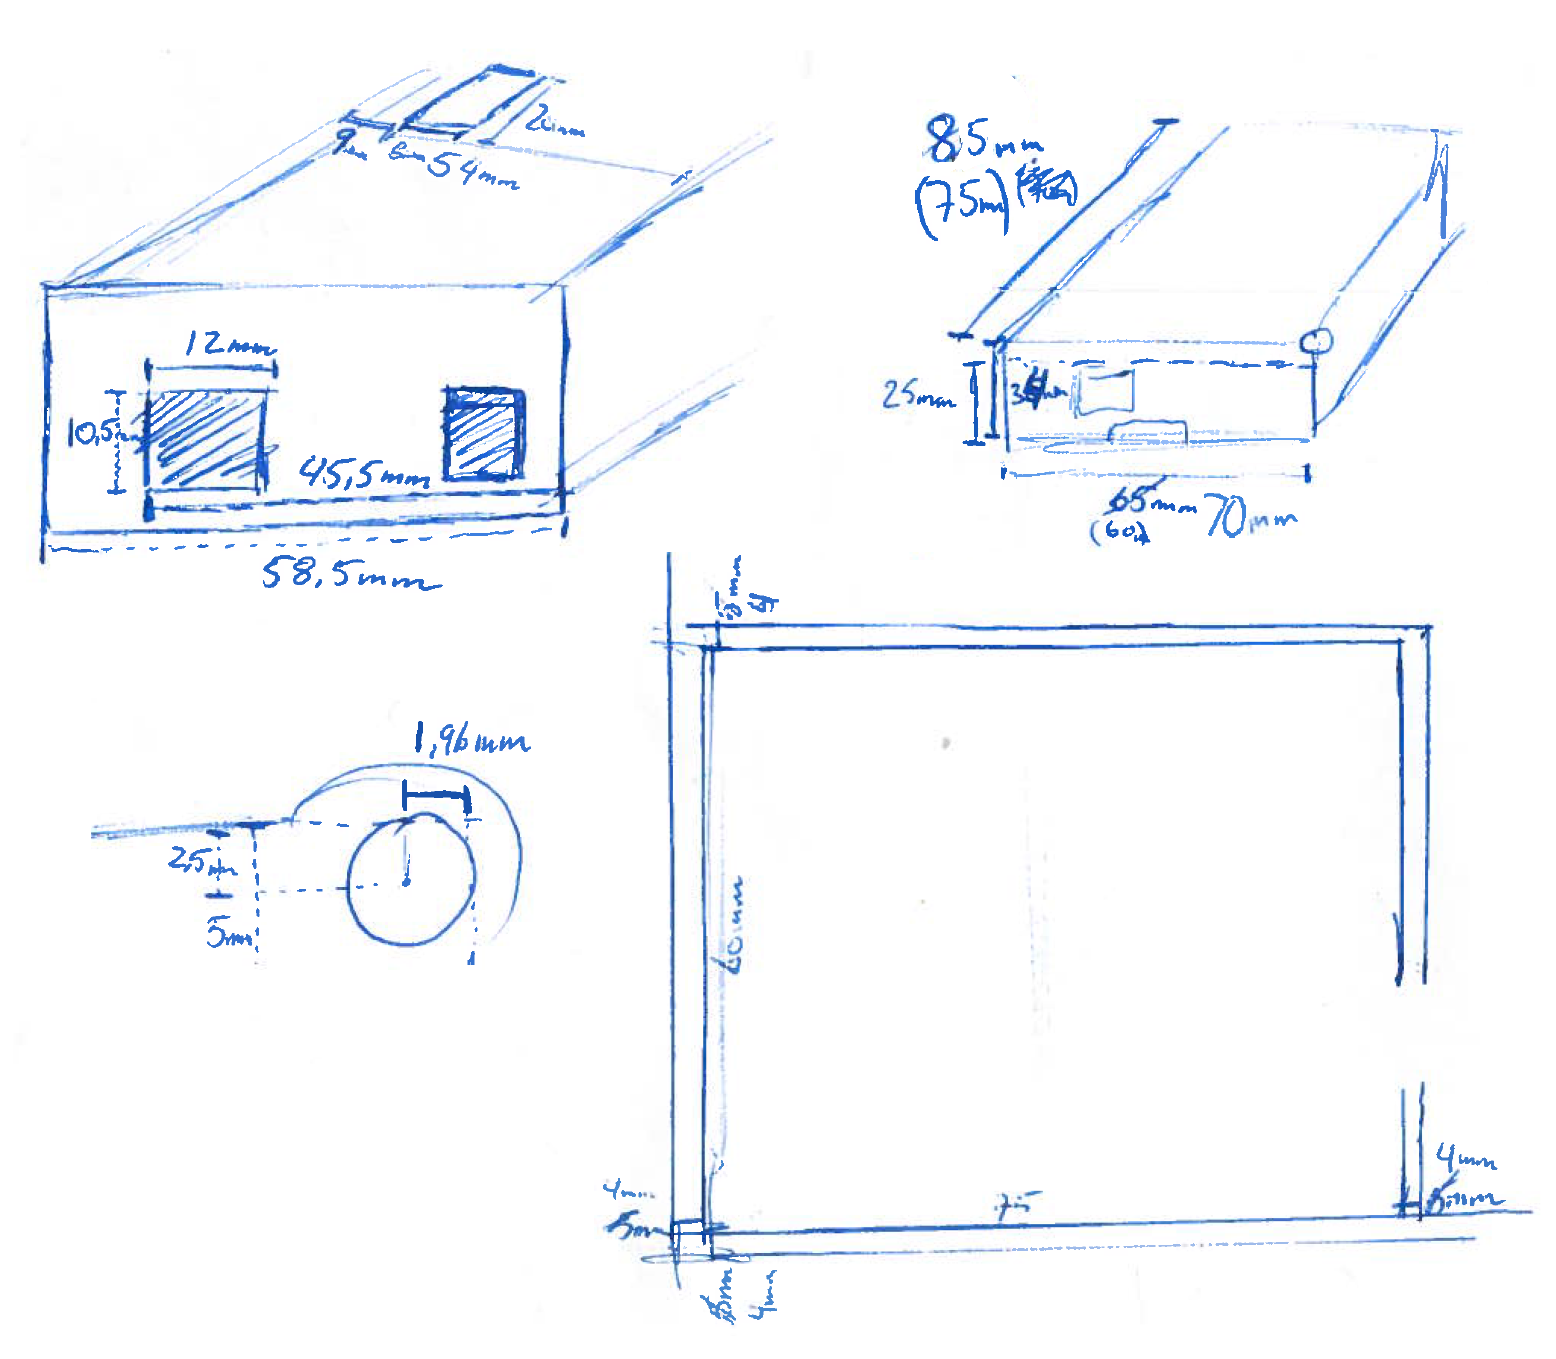
\includegraphics[width = \textwidth]{Figure/sketch_case.png}
\caption{The initial drawings of the case for the arduino. The drawing contains the rough measurements of the case. The measurements later got updated when it was not possible to get 5mm plywood. The design of the hinge is also shown in the bottom left.}
\label{fig:sketch_case}
\end{figure}

The hinge consists of a a semi circle with a hole in it. The purpose was to make a split on either side of the lid which would protrude into the hole allowing the lid to open and shut. The hinge is seen sketched on \autoref{fig:sketch_case}. 
\noindent
Afterwards a simple cardboard model was constructed in order to better visualise how the pieces could fit together. It was cut out from a cardboard box previously containing a set of head phones, hence the logo. The box is shown on \autoref{fig:rapid_model}. The simple cardboard model also served to confirm the previous measurements which were made and to make some adjustments as to where the hole for the wires and usb cable should be.


\begin{figure}[htb]
\centering
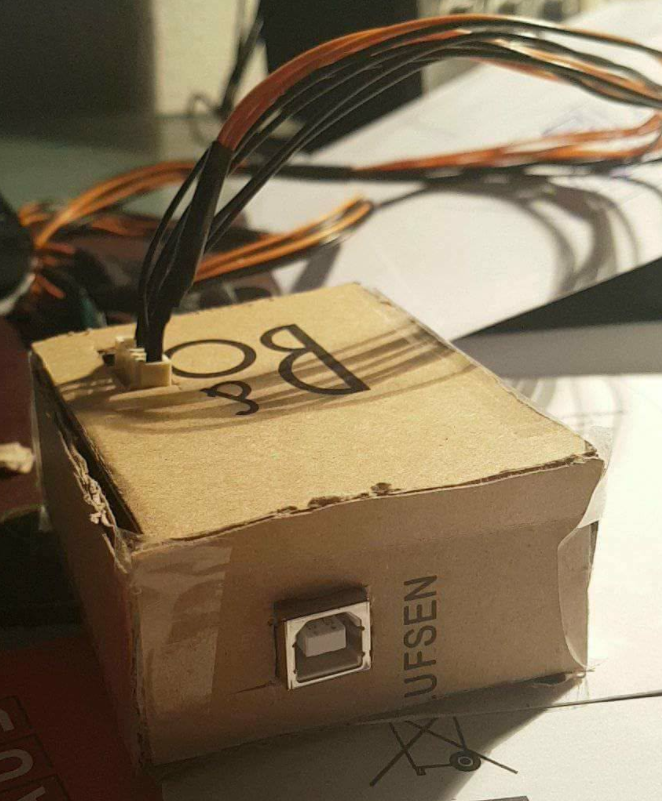
\includegraphics[scale=0.75]{Figure/rapid_model.png}
\caption{The rapid model constructed in card board before any vector drawing took place.}
\label{fig:rapid_model}
\end{figure}

\section{Preparing to lasercut}
We felt we were ready and began drawing the arduino case in Adobe Illustrator in order to get the Arduino case laser cutted.  It was assumed that we had access to 5mm plywood which later turned out not to be the case. The vector design had to be adjusted after this insight because the joints did not fit well any more. On \autoref{fig:vector_case} the finalised vector drawing of the arduino case is shown. The four sides are practically pairs of the same part with the exception of the end with the USB A/B hole in it. Additionally each pair was mirrored once due to the fact that the laser cutters left black sod on one side. This was done to avoid having sod on the outside.

\begin{figure}[htb]
\centering
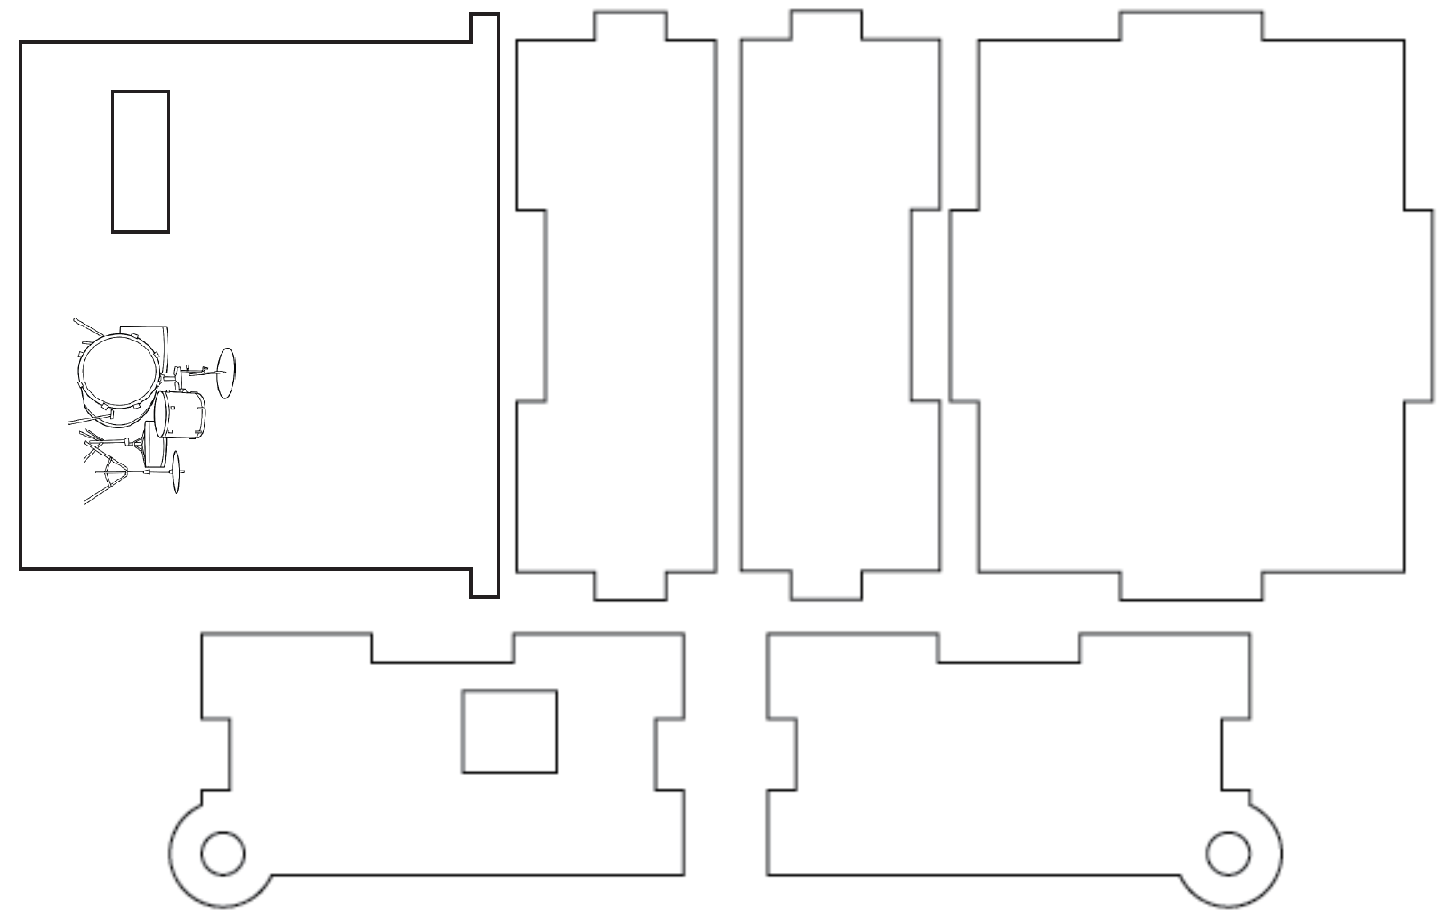
\includegraphics[width = \textwidth]{Figure/vector_case.png}
\caption{The enclosure for the arduino and shield as it was made in Adobe Illustrator. The stroke has been increased to 1 in order to better visualise the outlines. The group rasterized a vector image of a drum kit and added it on top of the lid.}
\label{fig:vector_case}
\end{figure}

The final measurements have been added to \autoref{fig:vector_measurement} in order to get a sense of the dimensions. It was a bit of a challenge to draw in 2D but think in 3D in order to visualise how the pieces should come together in the end.

\begin{figure}[htb]
\centering
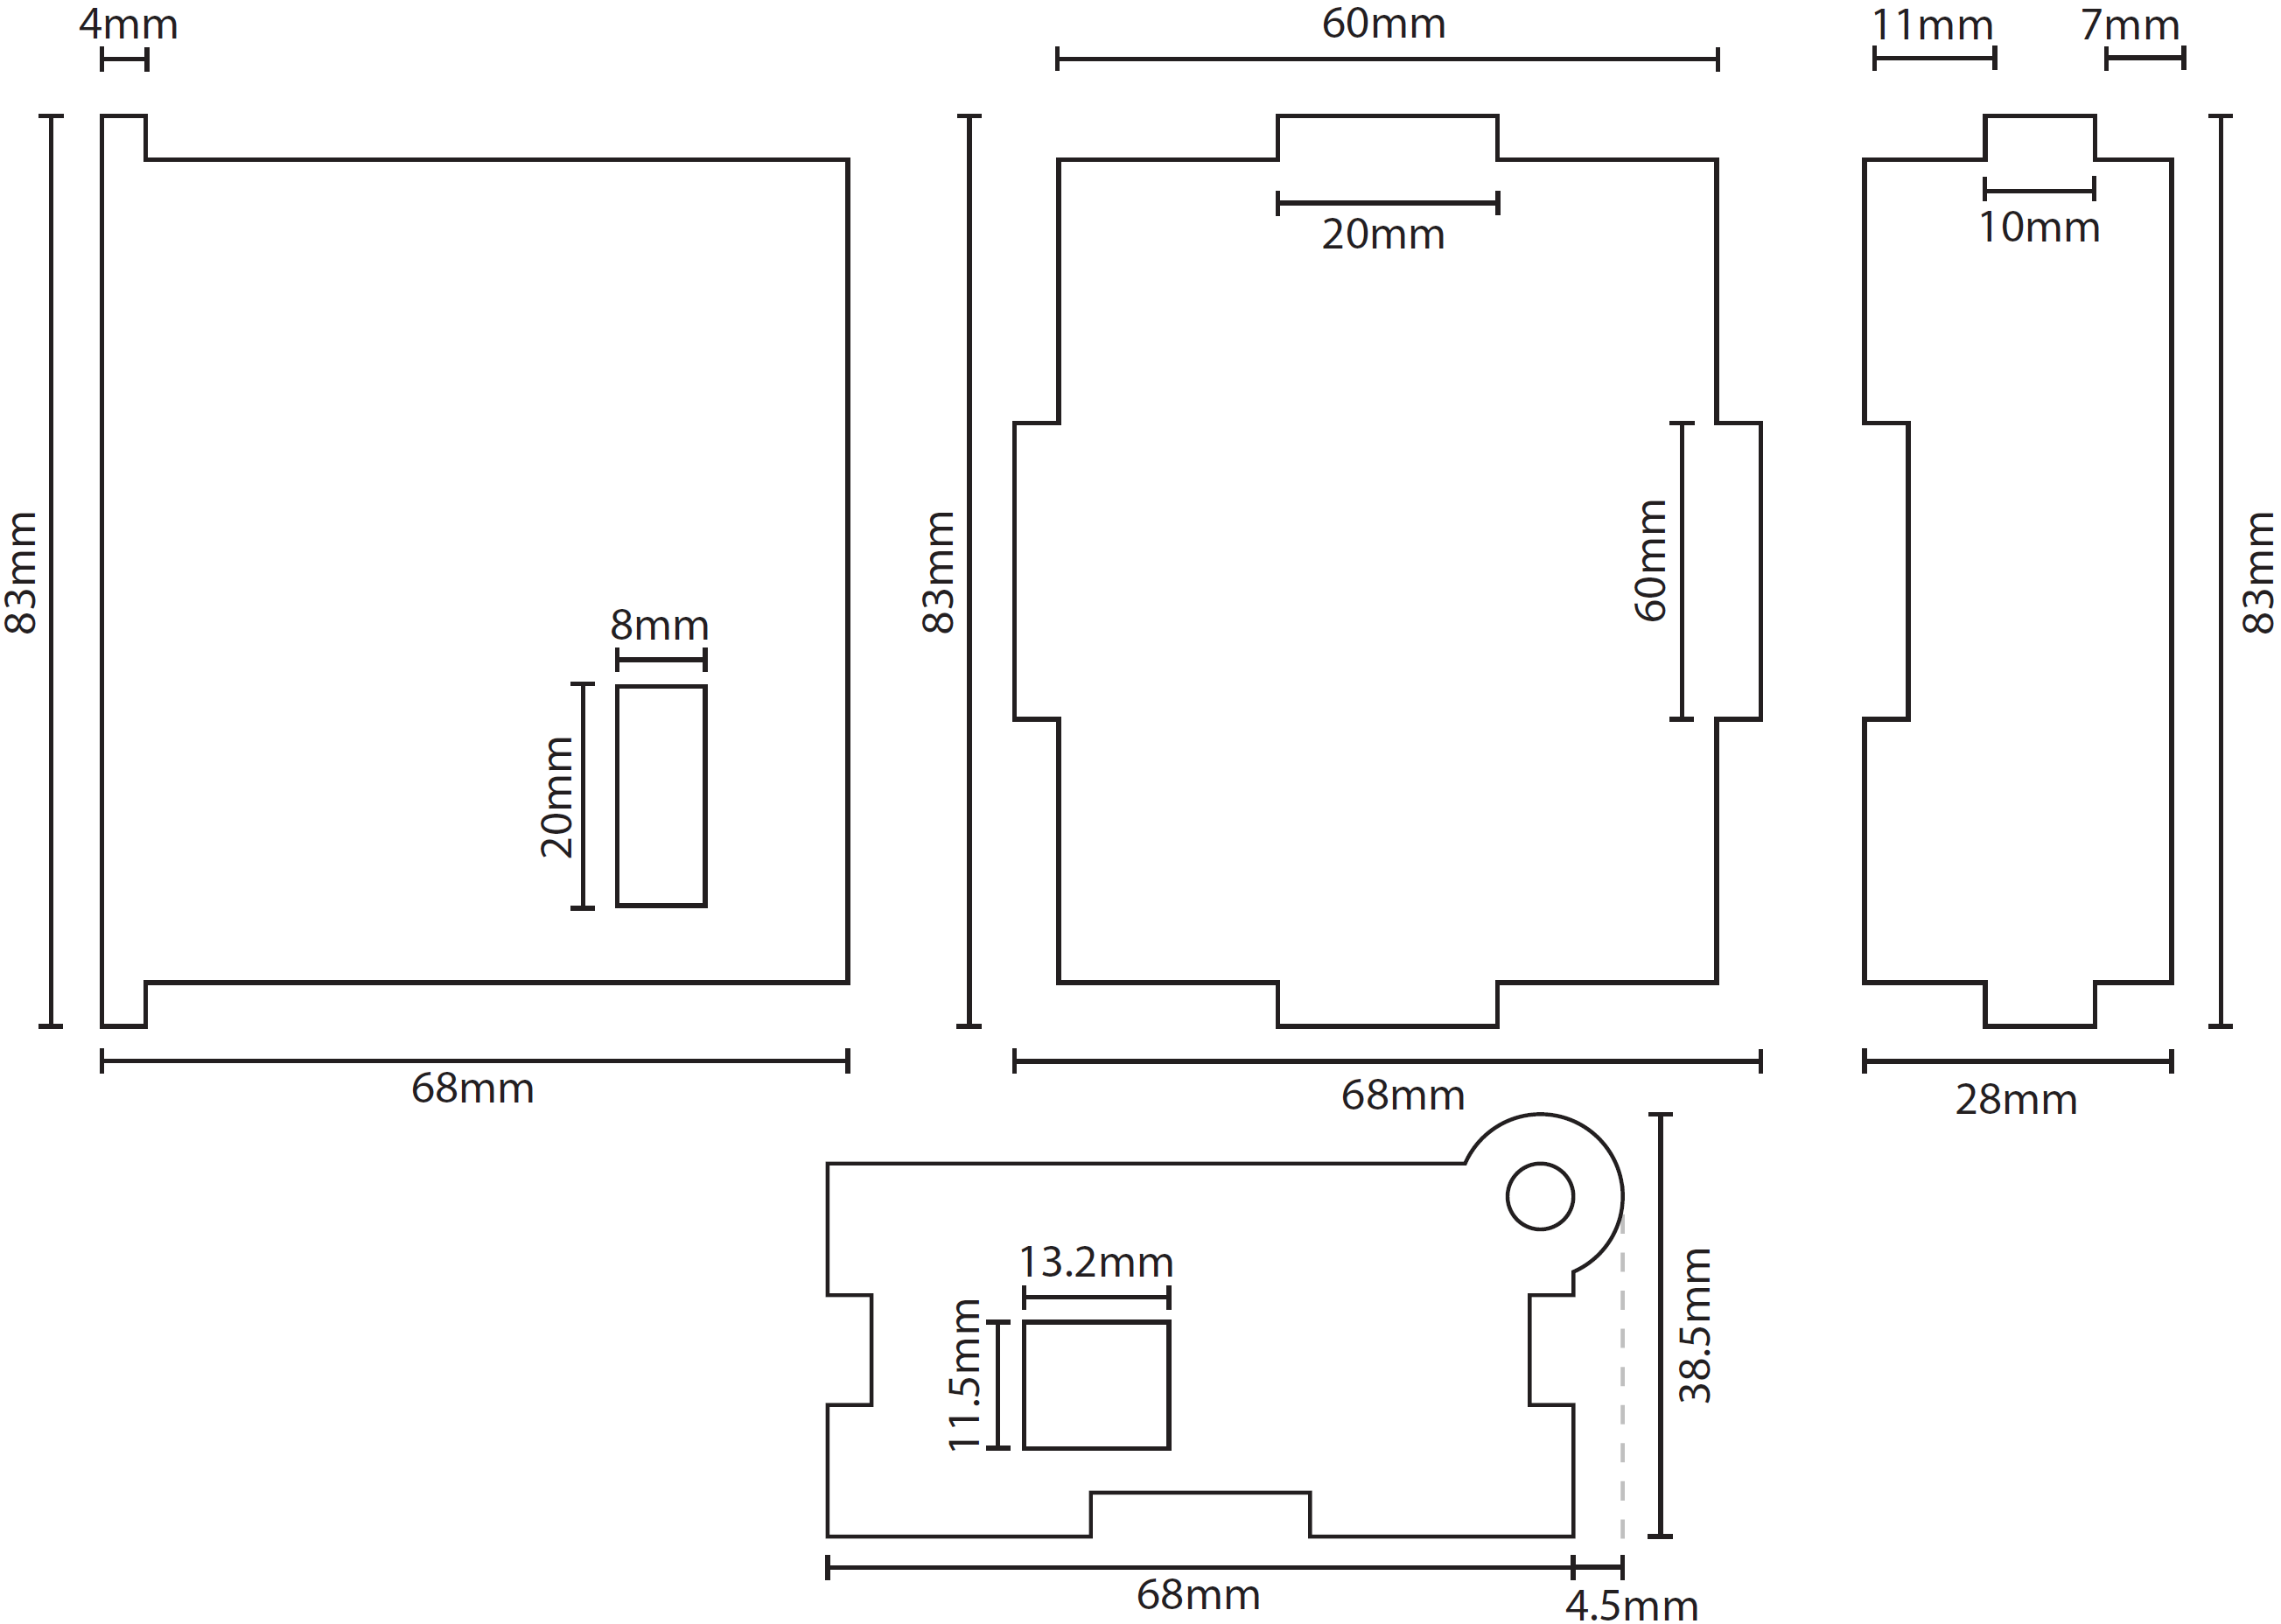
\includegraphics[width = \textwidth]{Figure/vector_case_measure.png}
\caption{The measurements on the vector drawing. It was decided to allow the Arduino some wiggle room.}
\label{fig:vector_measurement}
\end{figure}
